% Created by tikzDevice version 0.12.3.1 on 2021-04-02 15:25:29
% !TEX encoding = UTF-8 Unicode
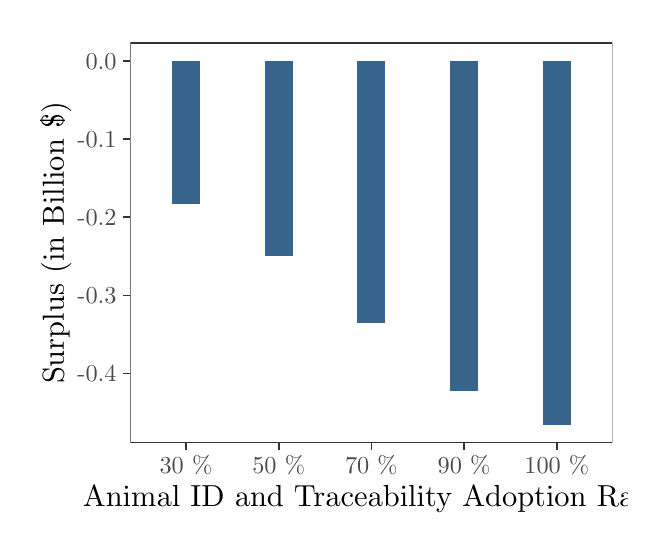
\begin{tikzpicture}[x=1pt,y=1pt]
\definecolor{fillColor}{RGB}{255,255,255}
\path[use as bounding box,fill=fillColor,fill opacity=0.00] (0,0) rectangle (216.81,180.67);
\begin{scope}
\path[clip] (  0.00,  0.00) rectangle (216.81,180.67);
\definecolor{drawColor}{RGB}{255,255,255}
\definecolor{fillColor}{RGB}{255,255,255}

\path[draw=drawColor,line width= 0.6pt,line join=round,line cap=round,fill=fillColor] (  0.00,  0.00) rectangle (216.81,180.68);
\end{scope}
\begin{scope}
\path[clip] ( 37.09, 30.69) rectangle (211.31,175.17);
\definecolor{fillColor}{RGB}{255,255,255}

\path[fill=fillColor] ( 37.09, 30.69) rectangle (211.31,175.17);
\definecolor{fillColor}{RGB}{54,100,139}

\path[fill=fillColor] ( 52.17,116.94) rectangle ( 62.22,168.61);

\path[fill=fillColor] ( 85.67, 98.26) rectangle ( 95.72,168.61);

\path[fill=fillColor] (119.17, 73.85) rectangle (129.22,168.61);

\path[fill=fillColor] (152.68, 49.44) rectangle (162.73,168.61);

\path[fill=fillColor] (186.18, 37.25) rectangle (196.23,168.61);
\definecolor{drawColor}{gray}{0.20}

\path[draw=drawColor,line width= 0.6pt,line join=round,line cap=round] ( 37.09, 30.69) rectangle (211.31,175.17);
\end{scope}
\begin{scope}
\path[clip] (  0.00,  0.00) rectangle (216.81,180.67);
\definecolor{drawColor}{gray}{0.30}

\node[text=drawColor,anchor=base east,inner sep=0pt, outer sep=0pt, scale=  0.88] at ( 32.14, 52.71) {-0.4};

\node[text=drawColor,anchor=base east,inner sep=0pt, outer sep=0pt, scale=  0.88] at ( 32.14, 80.92) {-0.3};

\node[text=drawColor,anchor=base east,inner sep=0pt, outer sep=0pt, scale=  0.88] at ( 32.14,109.14) {-0.2};

\node[text=drawColor,anchor=base east,inner sep=0pt, outer sep=0pt, scale=  0.88] at ( 32.14,137.36) {-0.1};

\node[text=drawColor,anchor=base east,inner sep=0pt, outer sep=0pt, scale=  0.88] at ( 32.14,165.58) {0.0};
\end{scope}
\begin{scope}
\path[clip] (  0.00,  0.00) rectangle (216.81,180.67);
\definecolor{drawColor}{gray}{0.20}

\path[draw=drawColor,line width= 0.6pt,line join=round] ( 34.34, 55.74) --
	( 37.09, 55.74);

\path[draw=drawColor,line width= 0.6pt,line join=round] ( 34.34, 83.95) --
	( 37.09, 83.95);

\path[draw=drawColor,line width= 0.6pt,line join=round] ( 34.34,112.17) --
	( 37.09,112.17);

\path[draw=drawColor,line width= 0.6pt,line join=round] ( 34.34,140.39) --
	( 37.09,140.39);

\path[draw=drawColor,line width= 0.6pt,line join=round] ( 34.34,168.61) --
	( 37.09,168.61);
\end{scope}
\begin{scope}
\path[clip] (  0.00,  0.00) rectangle (216.81,180.67);
\definecolor{drawColor}{gray}{0.20}

\path[draw=drawColor,line width= 0.6pt,line join=round] ( 57.19, 27.94) --
	( 57.19, 30.69);

\path[draw=drawColor,line width= 0.6pt,line join=round] ( 90.70, 27.94) --
	( 90.70, 30.69);

\path[draw=drawColor,line width= 0.6pt,line join=round] (124.20, 27.94) --
	(124.20, 30.69);

\path[draw=drawColor,line width= 0.6pt,line join=round] (157.70, 27.94) --
	(157.70, 30.69);

\path[draw=drawColor,line width= 0.6pt,line join=round] (191.21, 27.94) --
	(191.21, 30.69);
\end{scope}
\begin{scope}
\path[clip] (  0.00,  0.00) rectangle (216.81,180.67);
\definecolor{drawColor}{gray}{0.30}

\node[text=drawColor,anchor=base,inner sep=0pt, outer sep=0pt, scale=  0.88] at ( 57.19, 19.68) {30 \%};

\node[text=drawColor,anchor=base,inner sep=0pt, outer sep=0pt, scale=  0.88] at ( 90.70, 19.68) {50 \%};

\node[text=drawColor,anchor=base,inner sep=0pt, outer sep=0pt, scale=  0.88] at (124.20, 19.68) {70 \%};

\node[text=drawColor,anchor=base,inner sep=0pt, outer sep=0pt, scale=  0.88] at (157.70, 19.68) {90 \%};

\node[text=drawColor,anchor=base,inner sep=0pt, outer sep=0pt, scale=  0.88] at (191.21, 19.68) {100 \%};
\end{scope}
\begin{scope}
\path[clip] (  0.00,  0.00) rectangle (216.81,180.67);
\definecolor{drawColor}{RGB}{0,0,0}

\node[text=drawColor,anchor=base,inner sep=0pt, outer sep=0pt, scale=  1.10] at (124.20,  7.64) {Animal ID and Traceability Adoption Rate};
\end{scope}
\begin{scope}
\path[clip] (  0.00,  0.00) rectangle (216.81,180.67);
\definecolor{drawColor}{RGB}{0,0,0}

\node[text=drawColor,rotate= 90.00,anchor=base,inner sep=0pt, outer sep=0pt, scale=  1.10] at ( 13.08,102.93) {Surplus (in Billion \$)};
\end{scope}
\end{tikzpicture}
